\chapter{Related Work}
\label{chap:rel_work}

Before introducing moodboard-based input for 3D generative models, it is essential to understand the current landscape of 3D generation techniques and the control mechanisms that have emerged alongside them. This chapter examines the evolution of 3D generative architectures, the diverse conditioning strategies employed in both 2D and 3D domains, the orchestration frameworks that translate heterogeneous design inputs into model-compatible signals, and the multimodal alignment methods that enable intelligent content extraction and quality assessment.

The chapter is organized around four complementary perspectives. First, we trace the architectural evolution of 3D generative models from neural radiance fields to latent diffusion systems, as this progression fundamentally shapes what forms of control are feasible. Second, we examine control methodologies, both those operating through 2D conditioning and those directly manipulating 3D representations, to understand existing approaches for guiding generation. Third, we explore orchestration and alignment techniques, focusing on how heterogeneous inputs can be translated and structured to interface with modern generative systems. Finally, we discuss multimodal embedding models for retrieval and evaluation, which provide similarity measures for selecting relevant moodboard elements and assessing alignment between generated outputs and design intent.

\section{Evolution of 3D Generative Architectures}

The progression of 3D generative models can be understood through two major architectural waves: early approaches grounded in neural radiance fields and implicit representations, and recent systems operating directly in structured 3D latent spaces. This evolution fundamentally altered both the capabilities and the control mechanisms available to users.

Understanding this architectural trajectory is crucial for evaluating how moodboard-based control can be integrated into modern 3D generation systems. The shift from view-based optimization to direct latent-space manipulation represents more than an incremental improvement, it fundamentally changes where and how control signals can be injected. Early NeRF-based methods naturally accommodated image-space conditioning because generation itself operated through 2D supervision. While this allowed control mechanisms developed for 2D image synthesis to be leveraged, they often struggled with multi-view consistency since standard 2D priors lack intrinsic 3D awareness. Contemporary latent diffusion models, by contrast, reason explicitly about 3D structure within learned representations, demanding that control signals either be projected into these latent spaces or translated into compatible formats.

This section traces this evolution chronologically, examining how each generation of models approached the fundamental challenge of generating coherent 3D content and what control paradigms emerged as a consequence. We begin with neural radiance fields and their reliance on 2D diffusion priors, then examine the transition to direct 3D latent diffusion systems that form the foundation of current state-of-the-art approaches.

\subsection{Neural Radiance Fields and 2D Supervision}

Neural Radiance Fields (NeRF) \cite{mildenhall2020nerfrepresentingscenesneural} established a foundational paradigm for learning-based 3D reconstruction by representing scenes as continuous volumetric functions optimized through differentiable volume rendering. This image-space formulation created an opportunity to sidestep the fundamental scarcity of 3D training data.

\begin{figure}[H]
\centering
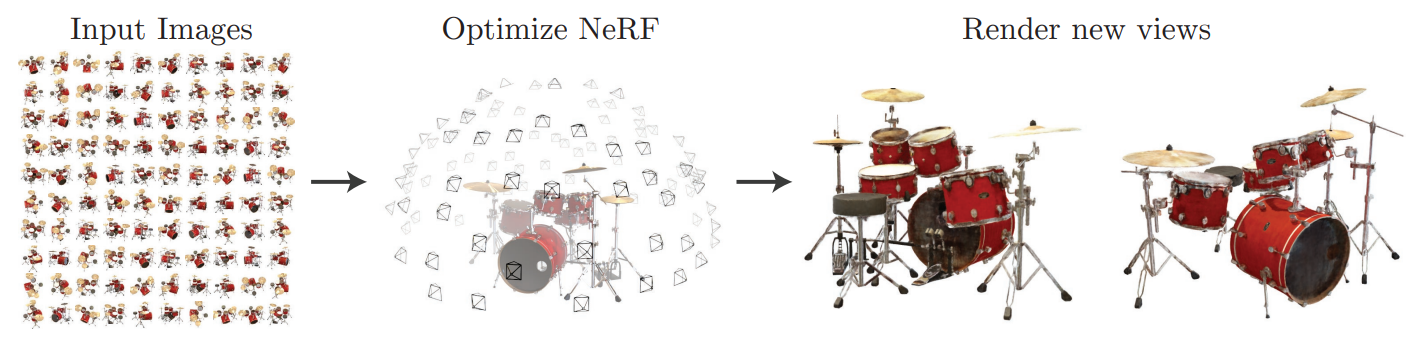
\includegraphics[width=0.95\textwidth]{images/nerf.png}
    \caption[NeRF overview]{NERF \cite{mildenhall2020nerfrepresentingscenesneural} optimizes a continuous volumetric scene function from a set of input images with known camera poses, enabling the generation of photorealistic novel views.}
\end{figure}

If 3D structure could emerge from 2D supervision, the powerful priors of text-to-image models could be directly leveraged to guide the optimization process. DreamFusion \cite{poole2022dreamfusiontextto3dusing2d} realized this potential by introducing Score Distillation Sampling (SDS). Instead of relying on ground-truth 3D data, SDS iteratively refines a NeRF by rendering views, adding noise, and using the noise estimates from a frozen 2D denoising U-Net to compute the update direction. This effectively distills 2D visual knowledge into explicit 3D structure.

\begin{figure}[H]
\centering
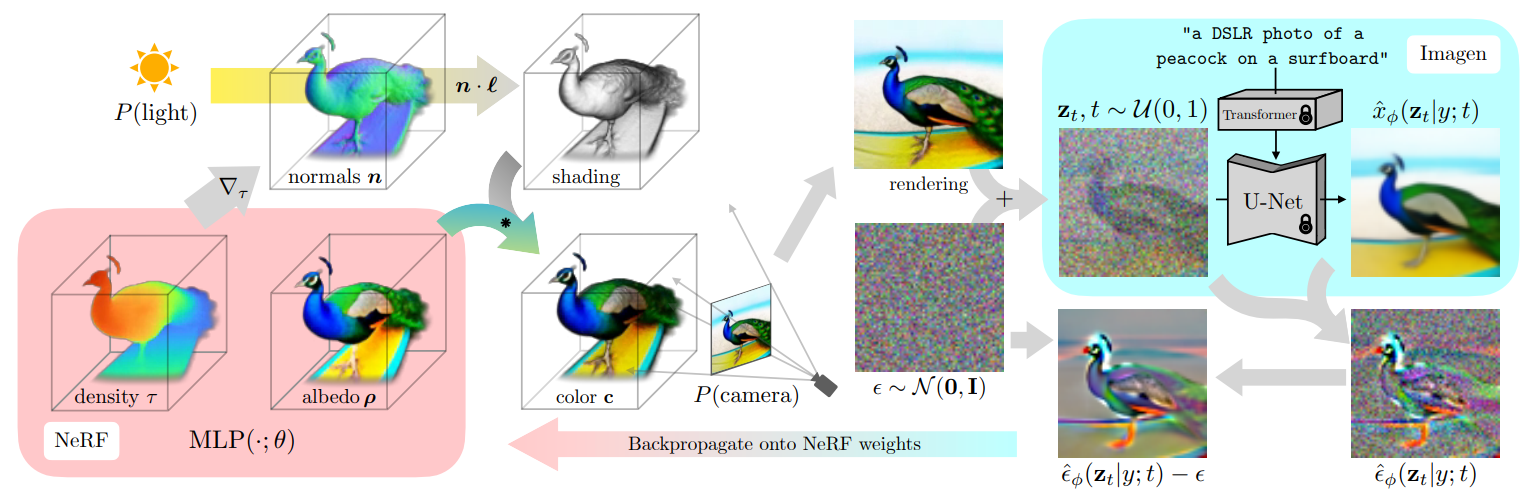
\includegraphics[width=0.95\textwidth]{images/dreamfusion.png}
    \caption[DreamFusion Overview]{DreamFusion \cite{poole2022dreamfusiontextto3dusing2d} optimizes a NeRF by rendering views, passing them through a frozen text-to-image diffusion model, and backpropagating the SDS gradient to refine geometry and appearance toward the text prompt.}
\end{figure}

While groundbreaking, early SDS introduced systematic biases resulting in "texture fog" and over-smoothed geometry. Subsequent research rapidly addressed these optimization pathologies. ProlificDreamer \cite{wang2023prolificdreamerhighfidelitydiversetextto3d} stabilized convergence and restored fine details with Variational Score Distillation (VSD). Magic3D \cite{lin2023magic3dhighresolutiontextto3dcontent} improved resolution limits via a coarse-to-fine pipeline, and Fantasia3D \cite{chen2023fantasia3ddisentanglinggeometryappearance} explicitly disentangled geometry from appearance to produce physically-grounded materials compatible with standard rendering engines.

Despite these iterative improvements, all methods operating through 2D supervision inherited two fatal constraints. First, per-scene optimization required minutes to hours, which precluded interactive design workflows. Second, and more critically, relying on 2D priors caused severe geometric inconsistencies across viewpoints. Because the 2D diffusion models guiding the generation lacked intrinsic 3D awareness, they frequently produced the "Janus problem" where objects generated with multiple faces or conflicting features on opposite sides. Approaches like MVDream \cite{shi2024mvdreammultiviewdiffusion3d} mitigated this by explicitly training diffusion models on synchronized multi-view images to enforce cross-view consistency, but the core representation remained implicitly image-centric.

Ultimately, these limitations catalyzed a fundamental architectural shift: moving away from multi-view 2D distillation and toward systems that treat geometry as a first-class, manipulable representation.

\subsection{Latent 3D diffusion models}

The limitations of view-based generation, namely geometric inconsistency, slow optimization, and implicit 3D reasoning, motivated a fundamental architectural shift. The most recent generation of 3D models abandons the image-centric paradigm to operate directly within explicit 3D latent spaces. Rather than coaxing 3D structure to emerge from multi-view rendering consistency, these systems treat geometry as a first-class representation where diffusion processes generate spatial content directly.

This transition required solving a representation problem with no clear 2D precedent. Unlike image latent spaces that efficiently compress pixel grids while preserving spatial structure, 3D extensions face inherent hurdles: naive volumetric grids scale cubically, and implicit NeRF representations lack the explicit structure required for efficient diffusion sampling. Consequently, recent systems have evolved from maximally flexible point-based representations to specialized hybrid architectures optimized for specific outputs.

The earliest attempts prioritized representational generality. 3DShape2VecSet \cite{zhang20233dshape2vecset3dshaperepresentation} represents shapes as neural fields built upon a learned set of vectors optimized for transformer processing. Its autoencoder accepts surface models and point clouds as input, encoding them into a set-based latent representation that captures both categorical identity and continuous stylistic variation. This transformer-friendly architecture preserves fine geometric details and enables multimodal conditioning (text, image, category), though the approach ultimately struggled to capture sharp edges and precise surface details.

\begin{figure}[H]
\centering
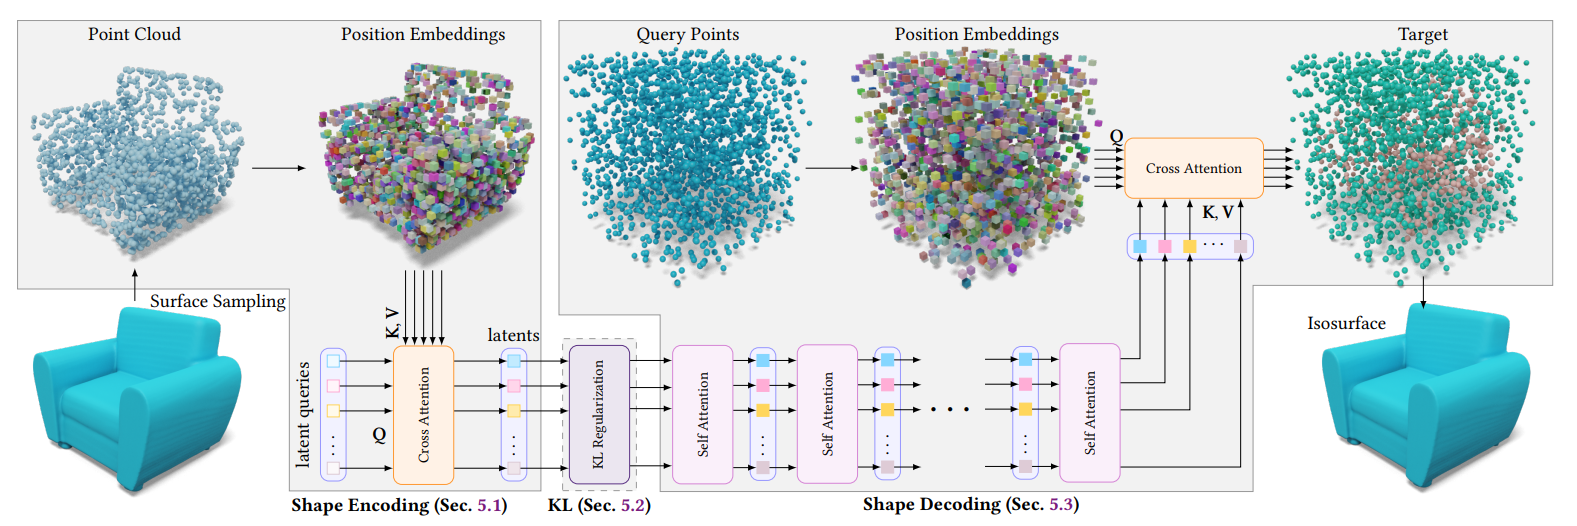
\includegraphics[width=0.95\textwidth]{images/3dshape2vecset.png}
    \caption[3DShape2VecSet Overview]{3DShape2VecSet \cite{zhang20233dshape2vecset3dshaperepresentation} has an autoencoder map heterogeneous 3D representations into a common embedding, enabling multimodal and category-aware 3D generation.}
\end{figure}

Building on this, Trellis \cite{xiang2025structured3dlatentsscalable} addresses the resolution-fidelity tension through its Structured LATent (SLAT) representation. SLAT uses a sparse 3D voxel grid to capture spatial occupancy, avoiding the memory cost of dense volumes while maintaining explicit spatial structure. Each occupied voxel carries visual embeddings extracted via self-supervised vision models (like DINOv2 \cite{oquab2024dinov2learningrobustvisual}). Diffusion operates jointly on geometric occupancy and visual features within this unified space. Critically, SLAT decouples generation from the output format, allowing the same encoding to be decoded into radiance fields, Gaussian splats, or explicit meshes.

\begin{figure}[H]
\centering
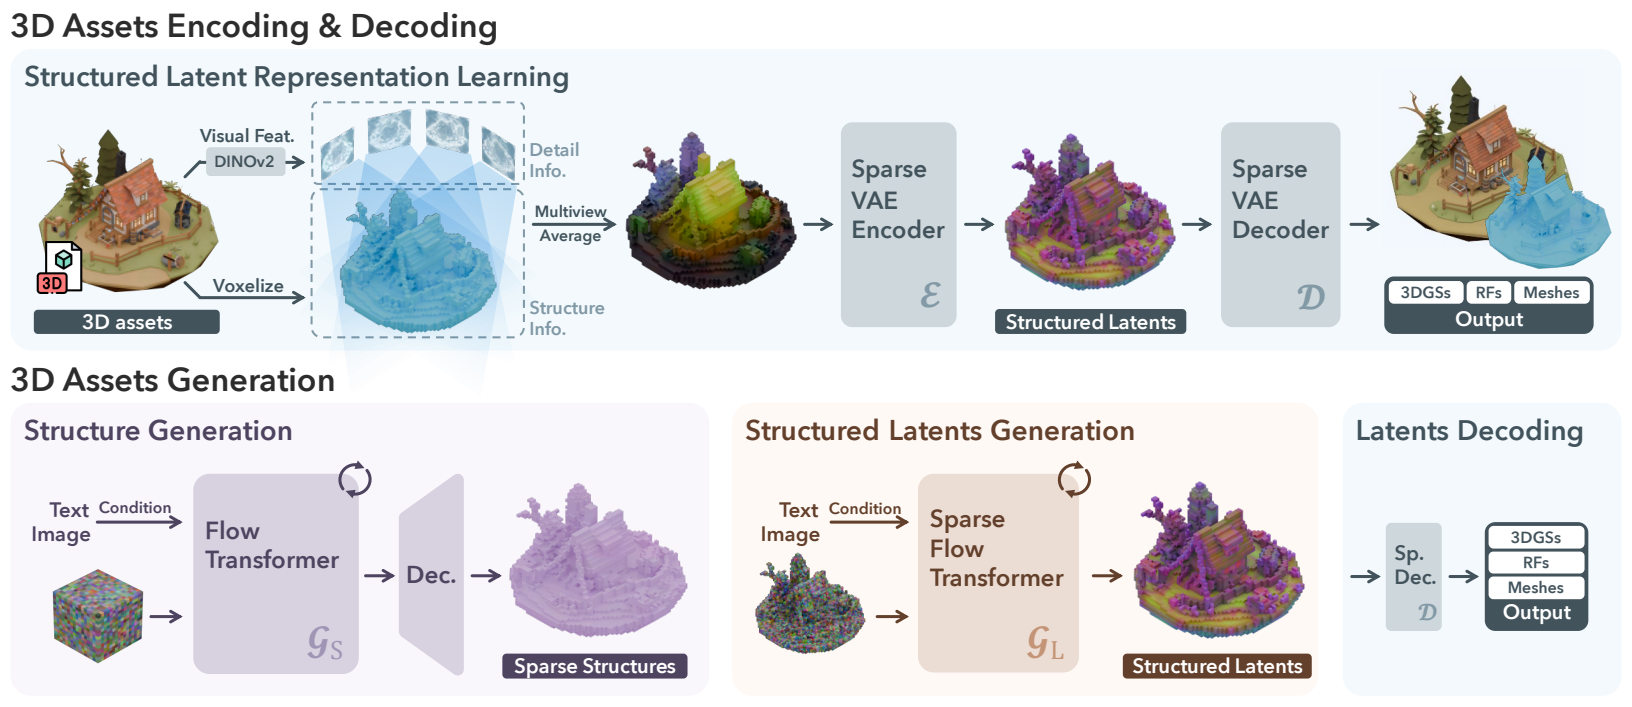
\includegraphics[width=0.95\textwidth]{images/trellis.png}
    \caption[Trellis Overview]{Trellis \cite{xiang2025structured3dlatentsscalable} augments a sparse voxel structure with visual features to enable joint geometry-appearance diffusion and flexible decoding into radiance fields, Gaussian splats, or meshes.}
\end{figure}

Where Trellis pursues architectural unification, Hunyuan3D 2.0 \cite{zhao2025hunyuan3d20scalingdiffusion} takes a compositional approach by decomposing generation into specialized sequential stages. A flow-based Diffusion Transformer first establishes the coarse geometry, such as silhouettes and proportions, from text or image inputs. A second stage then performs multi-view texture synthesis, generating consistent appearances while estimating physically-based rendering (PBR) parameters. This separation enables higher-resolution outputs by optimizing each stage independently, though it requires careful coordination to ensure the synthesized texture faithfully respects the predicted geometry.

\begin{figure}[H]
\centering
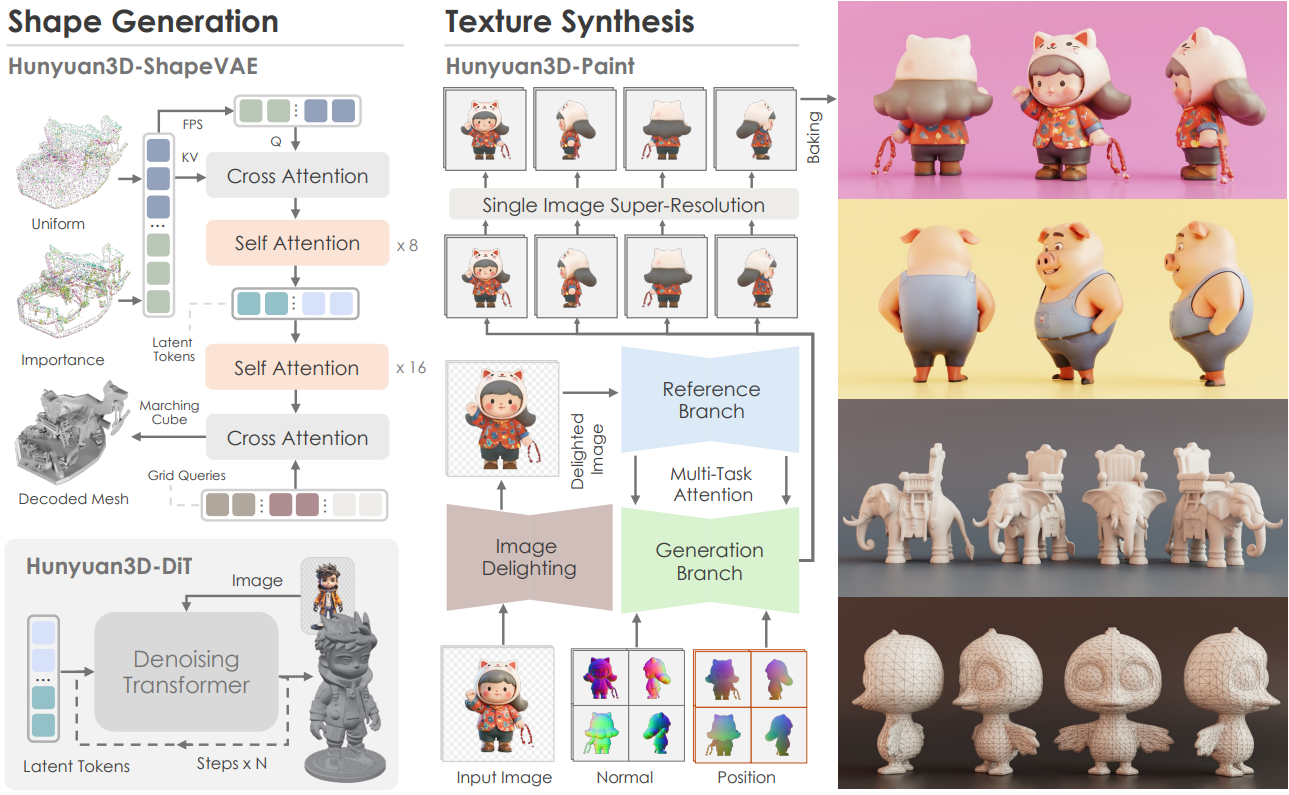
\includegraphics[width=0.95\textwidth]{images/hunyuan3d-2.0.png}
    \caption[Hunyuan3D 2.0 Overview]{Hunyuan3D 2.0 \cite{zhao2025hunyuan3d20scalingdiffusion} - A coarse shape predicted by a Diffusion Transformer is followed by a multi-view texture synthesis stage that outputs PBR materials and high-quality textures.}
\end{figure}

Ultimately, these latent 3D diffusion models achieve substantially stronger geometric coherence than their NeRF-based predecessors by reasoning explicitly about spatial structure. They largely eliminate artifacts like the Janus problem by enforcing geometric constraints directly. They also scale more effectively, utilizing latent spaces designed to capture 3D invariances and symmetries rather than inferring them implicitly from image statistics.

However, this architectural shift fundamentally complicates how control can be exercised. Without the rendering-based interfaces of NeRFs, 2D constraints like depth maps cannot be easily injected into a voxel or point cloud diffusion process. Control must instead operate through one of two pathways: learned latent-space adapters that project external signals directly into the 3D representation, or intelligent translation layers that convert diverse inputs into natively understood modalities. 

This distinction frames the two approaches explored in this thesis. The control approach extends latent 3D models with lightweight adapters, preserving fine-grained details but requiring paired training data. Conversely, the orchestration approach sidesteps the need for specific adapters by translating heterogeneous elements into combinations of text, images, and geometric primitives. While this sacrifices some representational fidelity, it exchanges it for broader applicability and reduced data requirements.

\section{Control Mechanisms in Generative Models}

Control mechanisms extend generative models beyond unconditional sampling by exposing explicit handles over structure, layout, style, or semantics. The primary challenge lies in translating a designer's intentions and visual references into structured inputs that generative models can process. This section traces the evolution of 2D control methods, from strictly spatial inputs to richer multimodal signals, and examines how these concepts extend into 3D latent-space control. Understanding the assumptions made by these architectures reveals critical gaps in current methodologies, specifically regarding why unstructured inputs like moodboards cannot simply be plugged into existing control frameworks.

\subsection{2D-Conditioned Control Methods}

The breakthrough that enabled practical control over diffusion models came from a simple architectural insight: rather than retraining large text-to-image models from scratch, lightweight adapter networks could be attached to frozen pretrained backbones. ControlNet \cite{zhang2023addingconditionalcontroltexttoimage} and compact alternatives like T2I-Adapter \cite{mou2023t2iadapterlearningadaptersdig} introduced parallel network branches that inject spatially aligned constraints, such as edge maps, depth, and pose, into the denoising process without disrupting the base model. While highly effective, these methods initially required training and loading separate models for every individual control modality.

\begin{figure}[H]
\centering
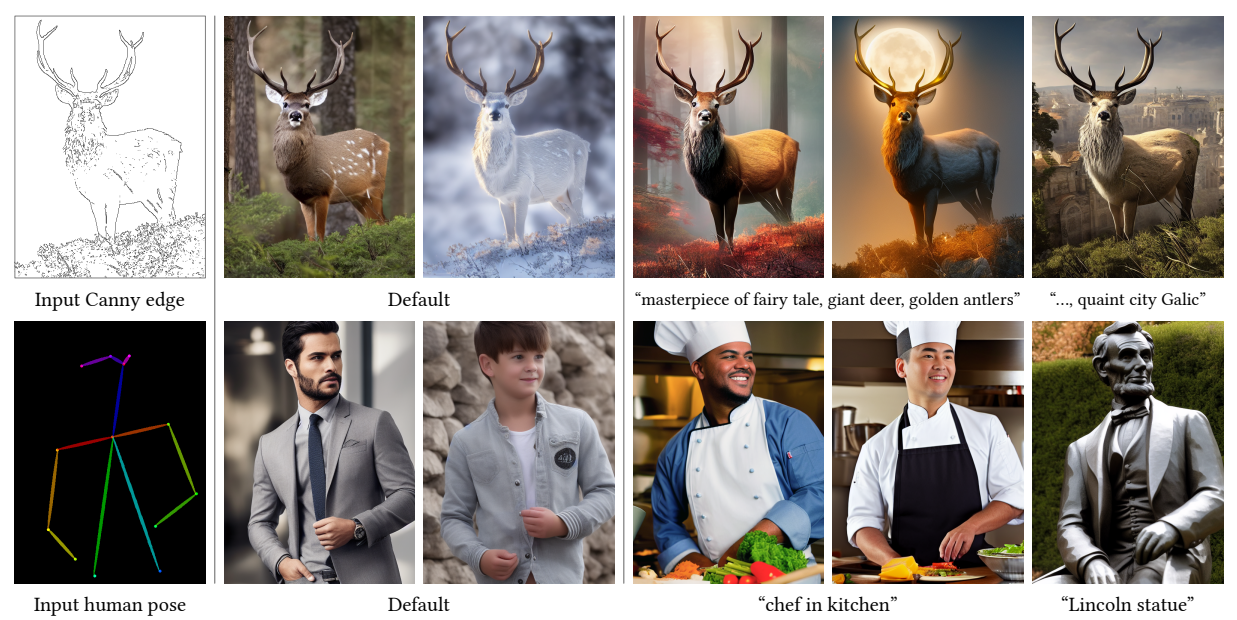
\includegraphics[width=0.95\textwidth]{images/controlnet.png}
    \caption[ControlNet Examples]{ControlNet \cite{zhang2023addingconditionalcontroltexttoimage} spatially guided image generation using edge and pose inputs.}
\end{figure}

To address this fragmentation, unified architectures like Uni-ControlNet \cite{zhao2023unicontrolnetallinonecontroltexttoimage} consolidated multiple spatial and global controls into a single backbone, dramatically reducing parameter counts. Crucially, the introduction of IP-Adapter \cite{ye2023ipadaptertextcompatibleimage} shifted control beyond strict spatial alignment. By decoupling cross-attention layers to process image features alongside text, IP-Adapter allowed reference images to act as direct conditioning prompts, enabling global stylistic and semantic features to guide generation fluidly.

\begin{figure}[H]
\centering
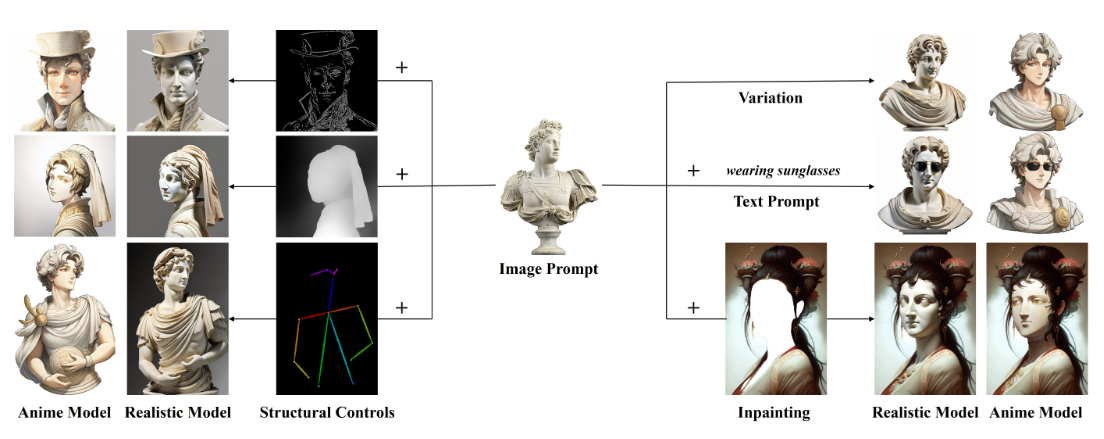
\includegraphics[width=0.95\textwidth]{images/ip-adapter.png}
    \caption[IP-Adapter Examples]{IP-Adapter \cite{ye2023ipadaptertextcompatibleimage} enables an image to act directly as a visual prompt, moving control away from strict spatial alignment and toward global stylistic and semantic guidance.}
\end{figure}

Other approaches focused on composition and abstract design. GLIGEN \cite{li2023gligenopensetgroundedtexttoimage} and training-free methods like BoxDiff \cite{xie2023boxdifftexttoimagesynthesistrainingfree} demonstrated that spatial layouts could be enforced via bounding boxes and attention manipulation. Moving even closer to intuitive design workflows, Brickify \cite{shi2025brickifyenablingexpressivedesign} replaced text prompts entirely with manipulable 2D design tokens, shifting control toward visual programming. Further extensions have successfully targeted abstract attributes, such as palette-based color guidance \cite{qiu2025exploringpalettebasedcolor}, and geometry integration via CAD-derived control maps \cite{ma2024generatingimages3dannotations}.

\begin{figure}[H]
\centering
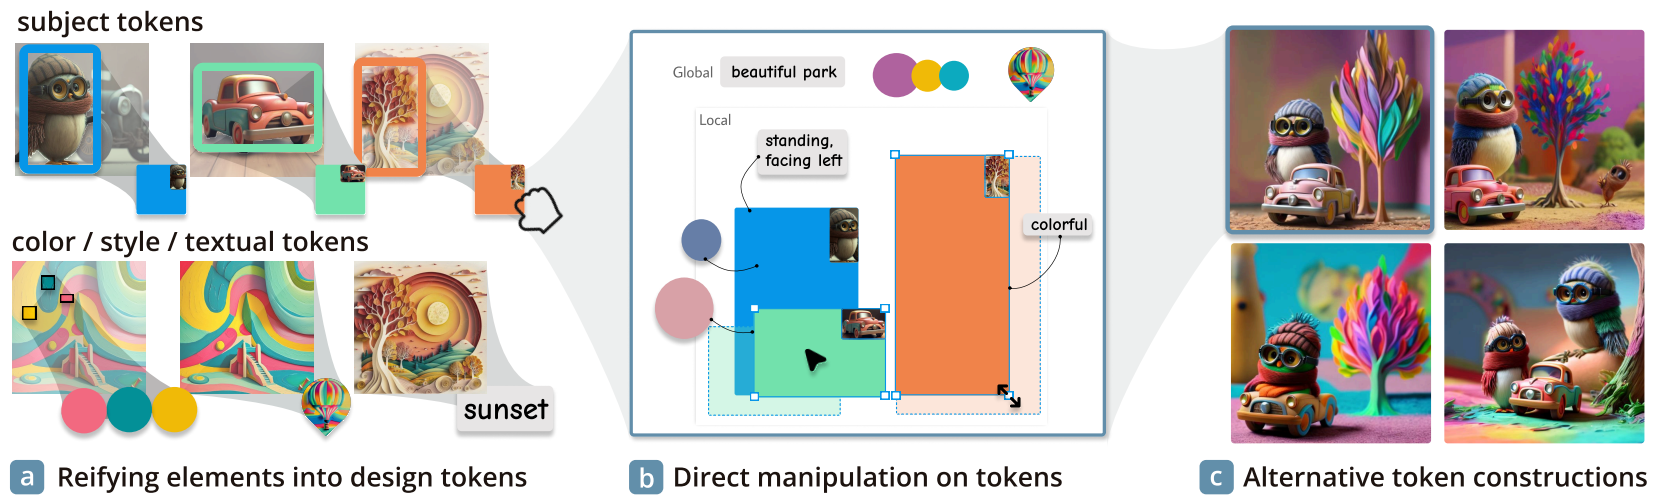
\includegraphics[width=0.95\textwidth]{images/brickify.png}
    \caption[Brickify Examples]{Brickify \cite{shi2025brickifyenablingexpressivedesign} enables explicit design control by manipulating visual tokens instead of text prompts.}
\end{figure}

Collectively, these 2D methods establish a robust toolkit for controllable image synthesis, but their success is fundamentally anchored to the image plane. Because they rely on strict spatial alignment, mapping 2D constraints like edge maps directly to 2D pixel grids, they cannot naturally enforce volumetric structure or multi-view consistency. An input that effectively constrains a single perspective offers no information about occluded geometry. Bridging this gap to 3D synthesis therefore requires abandoning planar assumptions and developing architectures capable of reasoning explicitly about spatial depth.

\subsection{3D-Aware Control Mechanisms}

Extending control mechanisms to 3D synthesis requires more than simply adding a Z-axis; it demands strict geometric coherence. Control signals must maintain absolute consistency across all viewpoints to ensure that constraints applied from one angle do not introduce contradictions elsewhere. Moreover, the control mechanism must be inherently compatible with the underlying 3D representation, whether an implicit field, mesh, or latent space, and the generation process must actively enforce spatial constraints in a way that pure 2D priors naturally fail to do.

\subsubsection{2D-Driven 3D Control Methods}

Early approaches to 3D control leveraged the existing Neural Radiance Field (NeRF) optimization framework by replacing or augmenting the 2D diffusion priors used for Score Distillation Sampling (SDS). Control3D \cite{chen2023control3dcontrollabletextto3dgeneration} builds on DreamFusion-style optimization but swaps the plain text-to-image diffusion model for a scribble-conditioned ControlNet. A differentiable sketch extractor renders the current NeRF state into edge maps, and a sketch-consistency loss encourages the 3D representation to match user-drawn contours. While this demonstrates that 2D control modules can guide 3D optimization, single-view scribbles provide weak geometric constraints, and the method inherits frequent view-consistency issues from its reliance on 2D priors.

\begin{figure}[H]
\centering
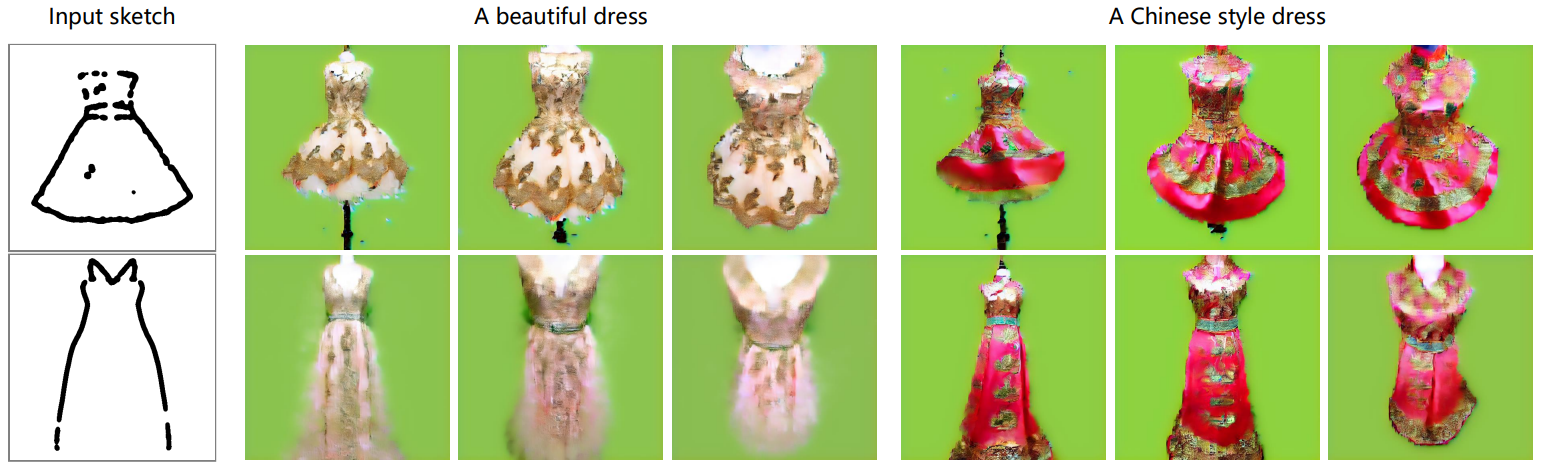
\includegraphics[width=\textwidth]{images/control3d.png}
    \caption[Control3D Examples]{Control3D \cite{chen2023control3dcontrollabletextto3dgeneration} uses a scribble-conditioned ControlNet and a sketch-consistency loss to guide NeRF-based 3D optimization.}
\end{figure}

To address these multi-view inconsistencies, ControlDreamer \cite{oh2024controldreamerblendinggeometrystyle} introduced explicit stage separation. A geometry stage first optimizes a NeRF using a multi-view diffusion model to establish consistent 3D structure, followed by a style stage that refines textures using an auxiliary Multi-View ControlNet conditioned on depth maps. MVControl \cite{li2023mvcontroladdingconditionalcontrol} generalized this multi-view conditioning by building a dedicated ControlNet directly on top of MVDream. It injects spatially aligned conditioning maps, edges, depth, normals, into a synchronized multi-view U-Net whose weights are shared across views. This ensures that an edge map from one angle correctly constrains the geometry visible in another.

\begin{figure}[H]
\centering
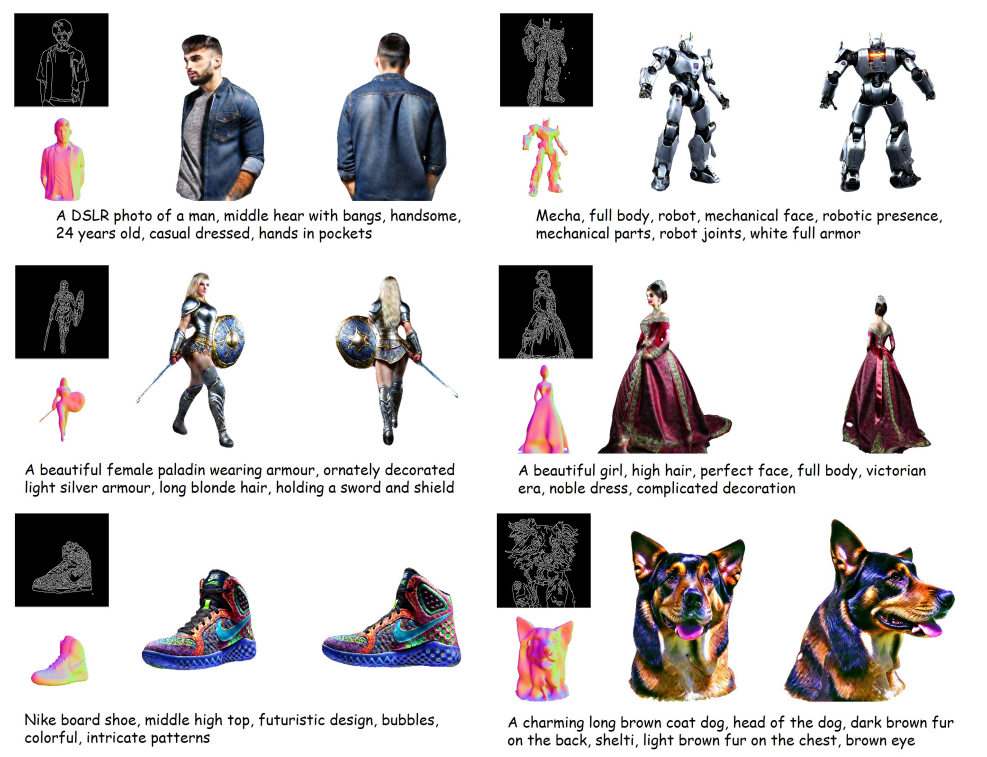
\includegraphics[width=\textwidth]{images/mvcontrol.png}
    \caption[MVControl Examples]{MVControl \cite{li2023mvcontroladdingconditionalcontrol} injects 2D control signals into a pose-aware multi-view U-Net, enforcing consistent constraints across viewpoints before lifting the results into a 3D Gaussian representation.}
\end{figure}

A fundamentally different direction emerged with feed-forward 3D generation systems that bypass iterative optimization entirely. CLAY \cite{zhang2024claycontrollablelargescalegenerative} predicts neural radiance fields directly from text or images in a single forward pass, integrating explicit control pathways into the generative architecture itself. Depth maps, semantic masks, and sparse geometry are encoded by dedicated control encoders and fused into the model through spatial cross-attention. While this represents a significant efficiency gain, CLAY still relies on explicit, well-structured conditioning inputs with known camera poses and does not generalize to abstract control sources.

\begin{figure}[H]
\centering
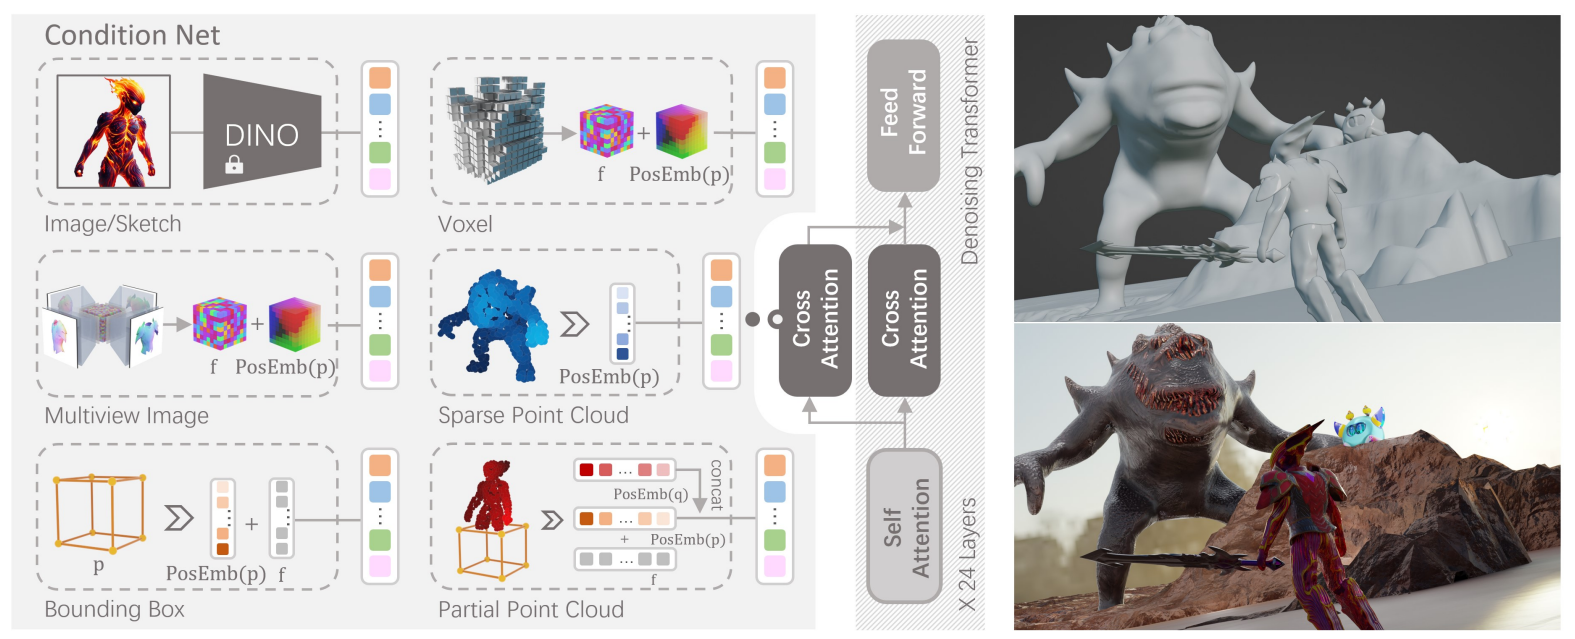
\includegraphics[width=\textwidth]{images/clay.png}
    \caption[CLAY Examples]{CLAY \cite{zhang2024claycontrollablelargescalegenerative} encodes diverse geometric and semantic controls and injects them via cross-attention into a feed-forward NeRF generator.}
\end{figure}

Other systems explored hybrid formulations. BiDiff \cite{ding2023textto3dgenerationbidirectionaldiffusion} proposes a bidirectional diffusion framework where a 2D image diffusion model and a 3D diffusion model run jointly, exchanging gradients so that texture and geometry mutually refine each other. Alternatively, text-to-3D pipelines based on video diffusion models, such as VFusion3D \cite{han2024vfusion3dlearningscalable3d}, treat multi-view renderings as short video sequences. By finetuning video diffusion backbones to produce 3D-consistent rotations, these systems apply temporal and multi-view constraints directly in diffusion space.

\subsubsection{Control in Learned 3D Latent Spaces}

The most recent generation of 3D control mechanisms operates directly in learned 3D latent spaces rather than through 2D projections. Hunyuan3D-Omni \cite{hunyuan3d2025hunyuan3domniunifiedframeworkcontrollable} exemplifies this shift by introducing a unified framework capable of ingesting diverse 3D control modalities, point clouds, voxels, skeletons, bounding boxes, through a single control encoder. It projects these heterogeneous representations into a common control space and injects them at appropriate stages of the generation pipeline, allowing the system to respond to structural constraints without requiring 2D multi-view map alignment.

\begin{figure}[H]
\centering
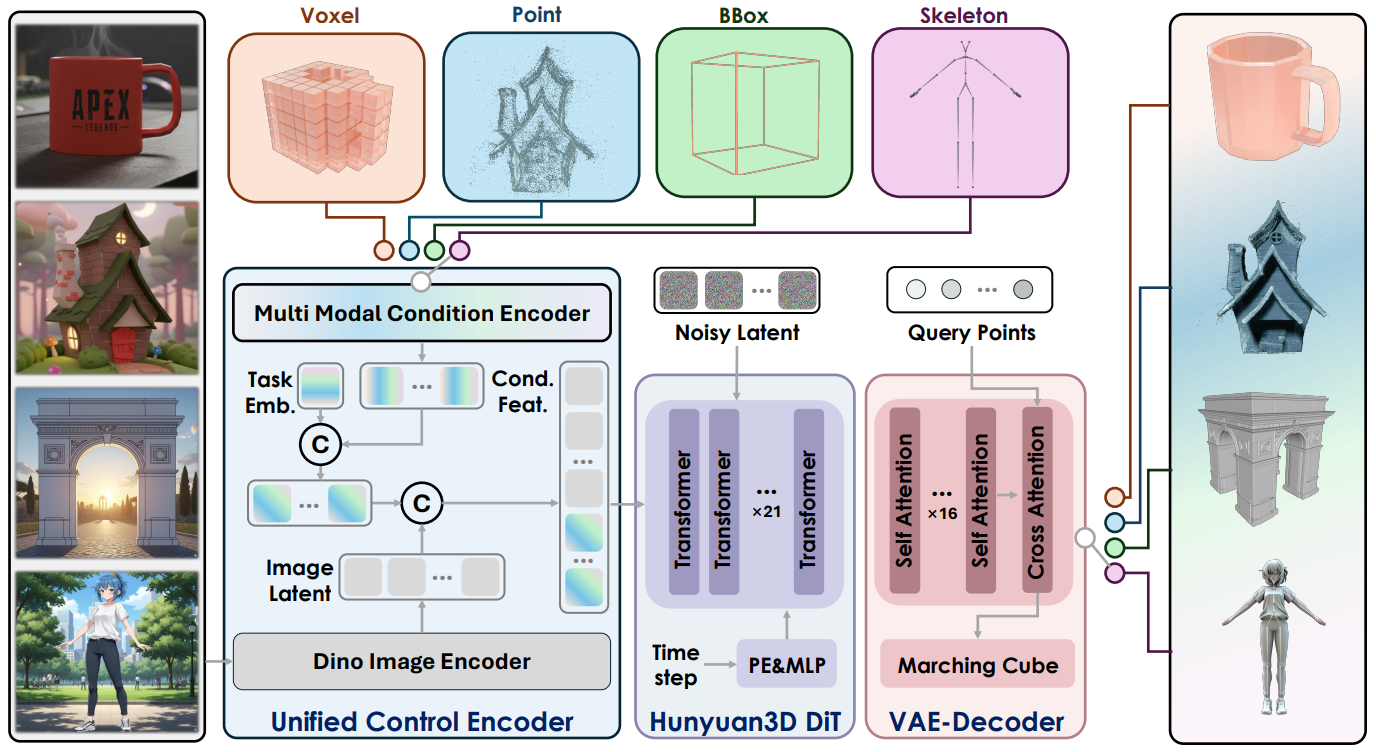
\includegraphics[width=\textwidth]{images/hunyuan3d-omni.png}
    \caption[Hunyuan3D-Omni Examples]{Hunyuan3D-Omni \cite{hunyuan3d2025hunyuan3domniunifiedframeworkcontrollable} integrates diverse 3D control modalities through a single multimodal encoder for diffusion-based 3D generation.}
\end{figure}

A complementary perspective treats control as multimodal conditioning within unified spaces. 3DShape2VecSet \cite{zhang20233dshape2vecset3dshaperepresentation} learns a point-cloud autoencoder whose latent vectors capture both category-level semantics and fine-grained geometry, while ShapeGPT \cite{yin2023shapegpt3dshapegeneration} tokenizes 3D shapes to align with text and images in a large multimodal transformer. Collectively, these 3D-aware mechanisms prove that strong geometric consistency and meaningful control are achievable, provided the control signals are explicit, structured, and paired with desired 3D outputs during training. 

\subsection{Limitations of Current Control Mechanisms}

Despite these architectural advancements, current 3D control frameworks fail when confronted with high-level, heterogeneous inputs like moodboards. This failure stems primarily from a fundamental representation space mismatch. Existing control mechanisms succeed precisely because they rely on inputs that share a direct, alignable coordinate space with the generated output. Just as a 2D bounding box maps precisely to pixel coordinates in an image, structured 3D controls like voxel grids, skeletons, and 3D bounding boxes map directly to the spatial geometry of a 3D asset. Moodboards, however, completely bypass this spatial alignment. They are inherently abstract, composed of loosely structured 2D images, floating color palettes, and textual concepts that lack any explicit coordinate mapping to the final 3D shape. Current architectures possess no native mechanism to inject a flat 2D color swatch or a non-spatial stylistic reference directly into a 3D latent space without a dedicated translation layer.

Compounding this representational mismatch is the significant challenge of data scarcity and the lack of automated extraction methods. Training dedicated control adapters for generative models requires massive datasets of paired inputs and target outputs. For standard control methods, conditioning signals can be automatically and synthetically extracted from existing 3D assets. Whether rendering 2D spatial constraints like depth maps and edge boundaries, or deriving 3D structural representations like voxel occupancy grids, point clouds, and surface normals, developers can algorithmically generate paired training data at an industrial scale. Moodboards offer no such automatable pathway. There is currently no reliable automated procedure for reverse-engineering a designer's abstract, multifaceted moodboard from a finished 3D asset. Manually curating such pairs is prohibitively expensive, meaning datasets at the scale required for direct adapter training are highly unlikely to exist in the foreseeable future. 

Because direct structural control is highly impractical under these constraints, this mismatch necessitates the alternative orchestration approaches explored in the following section. Rather than attempting to train new adapters for incompatible data structures, orchestration sidesteps the supervision problem entirely by interpreting and translating moodboard elements into the distinct textual and visual formats that existing generative models already understand.

\section{Orchestrating Heterogeneous Inputs}

The control mechanisms surveyed in the previous section demonstrate that generative models can accommodate diverse conditioning modalities. However, they share a critical limitation: they require control signals in specific formats with large-scale paired supervision. Many of these signals, such as depth or edge maps, can be generated automatically from source images. This allows existing systems to rely on datasets where the required targets are synthetically derived. Moodboards offer no such path. Their elements are heterogeneous, unstructured, and not directly convertible into the spatially aligned supervision signals that current control architectures expect. Because moodboards lack an automatable way to generate these paired targets, they cannot be plugged into existing control frameworks.

The orchestration approach sidesteps this supervision problem through intelligent translation rather than direct learning. Instead of training adapters that map moodboard content into model latent spaces, orchestration systems analyze and transform heterogeneous inputs into formats that existing generative models already understand, such as text prompts, reference images, and structured parameters. This strategy sacrifices some representational fidelity, as the translation process may lose nuanced relationships between elements, but it gains crucial advantages. It eliminates the need for paired datasets that do not exist. It enables immediate deployment with pretrained models without expensive retraining. Furthermore, it naturally composes with existing control mechanisms by leveraging their strengths while compensating for their format restrictions.

\subsection{Multi-Agent Decomposition}

The core of this orchestration paradigm relies on structured multi-agent decomposition. Rather than attempting a holistic learned mapping, this approach treats moodboard translation as a staged pipeline. It progressively converts heterogeneous elements into model-ready conditioning through transformation, organization, and synthesis. By leveraging the zero-shot reasoning capabilities of large language and vision models, this paradigm maintains modularity and interpretability while completely bypassing the need for paired 3D datasets.

LL3M \cite{lu2025ll3mlargelanguage3d} provides a compelling precedent for how complex translation emerges from structured decomposition. While LL3M addresses text-to-3D procedural modeling, its architecture illustrates how staged pipelines can resolve ambiguity, preserve interpretability, and distribute responsibilities across specialized components without relying on end-to-end training. Applying a similar multi-agent translation paradigm to moodboards emphasizes organization, selective filtering, and synthesis to convert a collection of design cues into actionable conditioning signals.

This decomposition approach offers critical practical strengths. It utilizes pretrained models and classical techniques rather than requiring domain-specific datasets. Each stage is completely transparent. Developers and users can inspect intermediate outputs, such as clustered embeddings, relevance scores, and synthesized prompts, to understand exactly how the system interpreted the moodboard constraints. Modules can evolve independently as better embedding models, tokenization schemes, or prompt-synthesis techniques become available. Backend adaptation also remains highly flexible, as only the final synthesis stage needs to change to support new generative 3D models.

At the same time, the staged architecture introduces inherent limitations. Each transformation boundary risks information loss, as the decomposition process can oversimplify subtle designer intent. Relevance filtering depends on similarity metrics that may not fully align with generative quality. Furthermore, the pipeline lacks end-to-end learning signals that could globally optimize it for final output fidelity.

Despite these constraints, multi-agent decomposition remains the most viable orchestration strategy for moodboard-driven generation. It provides a structured, transparent way to translate abstract, heterogeneous content into precise constraints. Most importantly, it satisfies the strict requirement of operating entirely without paired training data, establishing the foundational architectural approach adopted in this thesis.

\section{Multimodal Embeddings for Retrieval and Evaluation}

Both orchestration and control rely on two fundamental operations: retrieving relevant moodboard elements for a generation query, and evaluating whether the final output aligns with the designer's intent. The conventional approach to this cross-modal challenge relies on embedding models designed to measure semantic similarity across diverse content types like text, images, and 3D geometry. While powerful in theory, tracking the evolution of these architectures reveals why they ultimately lack the reliability required for nuanced design workflows.

\subsection{Vision-Language Models}

The foundation for cross-modal retrieval emerged with CLIP \cite{radford2021learningtransferablevisualmodels}, which demonstrated that large-scale contrastive learning could align text and image representations in a shared embedding space. However, CLIP's global contrastive loss created quadratic memory constraints and struggled with noisy captions. SigLIP \cite{zhai2023sigmoidlosslanguageimage} later resolved these scaling bottlenecks by treating image-text matching as independent binary classifications rather than multi-class comparisons. Because they were trained on massive web-scraped datasets, these 2D vision-language models achieved remarkable zero-shot reliability. Yet for 3D generation, a critical modality remained missing.

\subsection{3D-Aware Embeddings}

Aligning 3D geometry with text and images is inherently difficult because geometric representations lack the massive paired datasets available for 2D media. ULIP \cite{xue2023uliplearningunifiedrepresentation} and ULIP-2 \cite{xue2024ulip2scalablemultimodalpretraining} addressed this by using synthetic multi-view renders to align point clouds with pretrained vision-language spaces. While effective at broad categorization, they struggled to capture subtle stylistic variations. OpenShape \cite{liu2023openshapescaling3dshape} subsequently attempted to solve this stylistic collapse by scaling up training to over a million 3D objects with carefully curated hard negative mining, proving that 3D embeddings can approach fine-grained aesthetic sensitivity provided sufficient data is available.

\subsection{Omni-Modal Systems}

Real moodboards encompass more than just text, images, and 3D shapes. Training specialized pairwise alignments for every new modality creates fragmented embedding spaces. OmniBind \cite{wang2024omnibindlargescaleomnimultimodal} introduced a unified architecture to solve this, using lightweight adapters and a learned routing system to integrate multiple specialist encoders into a single cohesive space.

\begin{figure}[H]
\centering
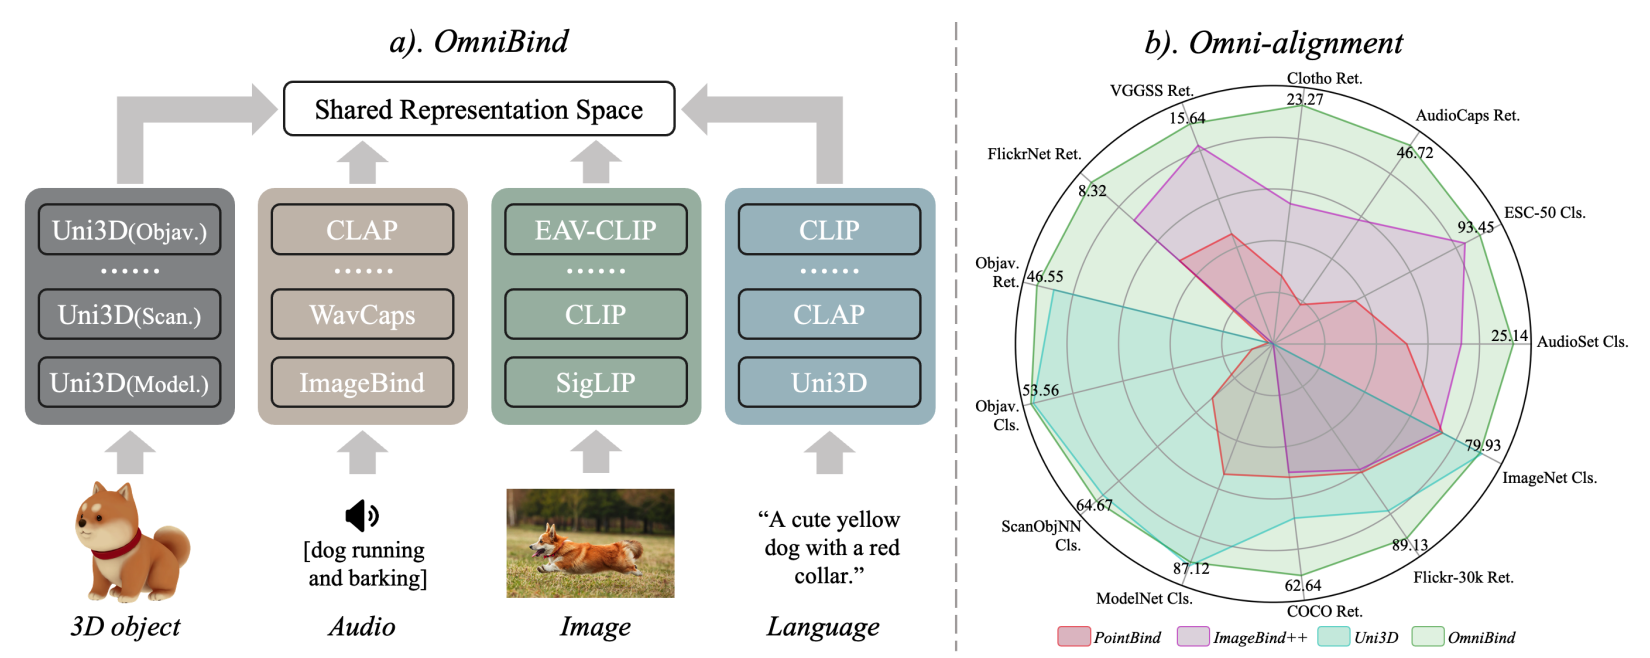
\includegraphics[width=\textwidth]{images/omnibind.png}
    \caption[OmniBind Overview]{OmniBind \cite{wang2024omnibindlargescaleomnimultimodal} integrates multiple specialist encoders into a shared embedding space using adapter projections and a learned Mixture-of-Experts router.}
\end{figure}

While systems like OmniBind exhibit fascinating emergent properties, they expose a critical vulnerability. As modalities increase and transition into 3D, these embedding architectures suffer a severe generalization penalty. Unlike CLIP, which reliably handles abstract concepts due to internet-scale training, 3D and omni-modal embeddings are constrained by limited or synthetic training distributions. When confronted with unseen data, highly niche design styles, or the abstract visual metaphors typical of human moodboards, their latent spaces become brittle. Calculating mathematical distance in these fragile, rigid latent spaces frequently yields unpredictable and unreliable retrieval results.

Because embedding-based systems cannot yet reliably interpret out-of-distribution design intent, this thesis abandons mathematical distance metrics in favor of an entirely different paradigm. Instead of relying on vulnerable spatial projections, the methodology relies on the robust, generalized zero-shot reasoning capabilities of massive vision-language models to semantically evaluate and organize moodboard content.